\documentclass[10pt]{article}

\usepackage[margin=0.68in]{geometry}
\usepackage[T1]{fontenc}
\usepackage[utf8]{inputenc}
\usepackage{lmodern}
\usepackage{microtype}
\usepackage{amsmath,amssymb}
\usepackage{booktabs}
\usepackage{tabularx}
\usepackage{array}
\usepackage{graphicx}
\usepackage{xcolor}
\usepackage{caption}
\usepackage{float}
\usepackage{enumitem}
\usepackage{listings}
\usepackage{tikz}
\usetikzlibrary{arrows.meta,positioning,fit,shapes.geometric}
\usepackage{multicol}
\usepackage{titlesec}
\usepackage[hidelinks]{hyperref}

\graphicspath{{images/}}
\captionsetup{font=small,labelfont=bf,skip=3pt}
\setlength{\parindent}{0pt}
\setlength{\parskip}{0.25em}
\setlength{\columnsep}{0.45cm}
\renewcommand{\arraystretch}{1.08}
\newcolumntype{Y}{>{\raggedright\arraybackslash}X}
\newcolumntype{R}[1]{>{\raggedleft\arraybackslash}p{#1}}
\raggedbottom

\titleformat{\section}{\large\bfseries}{\thesection}{0.55em}{}
\titleformat{\subsection}{\normalsize\bfseries}{\thesubsection}{0.50em}{}
\titleformat{\subsubsection}{\normalsize\itshape}{\thesubsubsection}{0.45em}{}
\titlespacing*{\section}{0pt}{0.65em}{0.30em}
\titlespacing*{\subsection}{0pt}{0.45em}{0.20em}
\titlespacing*{\subsubsection}{0pt}{0.35em}{0.15em}

\definecolor{codebg}{RGB}{247,247,247}
\definecolor{codeframe}{RGB}{180,180,180}
\lstset{
  basicstyle=\ttfamily\scriptsize,
  columns=fullflexible,
  frame=single,
  rulecolor=\color{codeframe},
  backgroundcolor=\color{codebg},
  xleftmargin=0.25em,
  xrightmargin=0.25em,
  aboveskip=0.35em,
  belowskip=0.35em,
  showstringspaces=false,
  breaklines=true
}

\newcommand{\todoresult}[1]{\textit{[Final experiment value to insert: #1]}}
\newcommand{\figureplaceholder}[3]{%
  \begin{figure}[H]
    \centering
    \fbox{\parbox[c][#1][c]{0.93\linewidth}{\small\raggedright
      \textbf{Experimental figure placeholder.} #2}}
    \caption{#3}
  \end{figure}%
}

% Title block is written explicitly to guarantee stable line breaks.
\begin{document}
\begin{center}
  {\LARGE\bfseries Routly Planner: Scalable PDDL+ Urban Routing\par}
  \vspace{0.25em}
  {\large Model-side compilation, controller-side replanning, and route-unaware LLM disruptions\par}
  \vspace{0.9em}
  {\normalsize Author Name \hspace{4.5em} Collaborator Name\par}
  \vspace{0.65em}
  {\normalsize July 2026\par}
\end{center}
\vspace{-0.3em}

\begin{abstract}
Routly Planner is an end-to-end framework for urban route planning over real
OpenStreetMap networks. OSMnx builds a directed road graph, ENHSP solves a
PDDL/PDDL+ problem, and SUMO validates the resulting route in a microscopic
traffic simulation. The domain includes traffic-dependent travel costs,
traffic lights, road availability, and optional fuel constraints. These
features improve realism, but they also expose the planner to large products of
roads, locations, numeric states, and temporal windows. Routly studies two
complementary scalability strategies. The \emph{model-side} branch replaces
unnecessary mid-road dynamics with compiled numeric traversal, changes the
state representation when appropriate, and precompiles valid actions with
singleton types; global congestion windows, hybrid temporal selection, and a
reversible macro-road abstraction further reduce the symbolic problem. The
\emph{controller-side} branch retains the expressive PDDL+ process model but
solves and joins smaller partial plans for congestion or fuel. A separate LLM
layer generates structured closures and slowdowns using topology and
start/goal information while remaining blind to the baseline route; a second
planner call measures route adaptation. In a verified 500-node Bologna case,
a generic dynamic encoding failed during grounding with an 8~GB Java heap,
whereas singleton-typed compilation produced a complete plan. All modelling
choices and experimental parameters are recorded through validated YAML
configuration snapshots.
\end{abstract}
\vspace{-0.35em}
\noindent\textbf{Keywords:} PDDL+; numeric planning; urban routing; grounding;
traffic congestion; replanning; large language models.

\section{Problem Description and Research Questions}

\subsection{Urban routing testbed}
Routly receives a directed road graph $G=(L,R)$, a vehicle $v$, a start
location $s$, and a goal location $g$. It must produce a feasible route that
minimises a numeric metric while respecting road availability and optional
time- and resource-dependent constraints. The current experimental target is
the drivable network of Bologna, Italy, queried from OpenStreetMap through
OSMnx. OSMnx constructs a directed multigraph and simplifies its topology by
removing interstitial geometry nodes while preserving actual junctions,
dead-ends, connectivity, and edge geometries \cite{boeing2017,boeing2025}.
Routly then applies a controlled crop radius (\texttt{distance\_meters}), a
maximum graph size (\texttt{max\_nodes}), connected-component filtering, and a
fixed seed. For each graph size, the benchmark stores and reuses one start/goal
pair near opposite parts of the sampled network, so comparisons change the
planning model rather than the route endpoints.

Bologna is a useful controlled case because its historic centre combines
radial corridors, a dense secondary street fabric, and a surrounding ring
structure. This produces both high-centrality corridors and plausible detours,
which are useful for studying congestion and road disruptions
\cite{nardino2021}. The city is not claimed to represent every urban
morphology; it is a reproducible case study whose graph can be expanded from
small to progressively larger instances.

The pipeline deliberately separates decision and simulation. PDDL/PDDL+ is the
decision layer, ENHSP performs grounding and search, and SUMO simulates the
chosen route together with background vehicles. SUMO is therefore a
microscopic validation and visualisation layer rather than the route optimiser
\cite{lopez2018}.

\subsection{Why a planner rather than only shortest-path search?}
Specialised graph algorithms such as Dijkstra, A*, and time-dependent routing
methods are extremely effective for shortest-path queries
\cite{baum2015}. They can also support traffic-dependent weights. The motivation
for PDDL+ is not that graph routing is incapable of representing traffic; it is
that a declarative planning model can combine heterogeneous logical, numeric,
and temporal requirements in one domain. PDDL+ distinguishes agent-controlled
actions, continuous processes, and autonomous events, making it natural to
model movement, time, fuel consumption, signal phases, and external
interruptions \cite{foxlong2006}. Prior work has already demonstrated PDDL+ for
macroscopic urban traffic control, particularly for adapting traffic-light
green phases \cite{vallati2016}. Routly instead focuses on the route of an
individual vehicle over an automatically extracted road network.

\begin{table}[H]
\centering
\caption{Realistic features and the planning burden they introduce.}
\label{tab:realism}
\small
\begin{tabularx}{\linewidth}{@{}p{2.5cm}Y Y@{}}
\toprule
Feature & Domain role & Main scalability effect \\
\midrule
Congestion & Road cost depends on background traffic and optionally on time. & Road/window values, additional numeric expressions, and temporal parameters. \\
Traffic lights & Expected delay depends on signal phases and intersection complexity. & Additional temporal cost and, in the process model, autonomous dynamics. \\
Fuel & Limited autonomy, discrete or continuous consumption, and refuelling. & Numeric preconditions/effects and intermediate station choices. \\
Road disruptions & Incidents, works, closures, and slowdowns alter availability or travel cost. & Alternative-route search and repeated planning under modified initial facts. \\
\bottomrule
\end{tabularx}
\end{table}

The same features that make the problem more realistic also enlarge the
symbolic and numeric instance. Numeric planning is highly sensitive to model
formulation, and PDDL+ deployment is constrained by a comparatively small
planner ecosystem \cite{scala2016,piotrowski2024}. Sparse topological relations
are particularly problematic when a generic action exposes many parameter
combinations to the grounder, even though very few are reachable or meaningful
\cite{franco2019}. Routly therefore treats \emph{modelling granularity} as the
central research problem.

\subsection{Research questions}
\begin{description}[leftmargin=1.05cm,labelwidth=0.85cm,itemsep=0.15em,topsep=0.1em]
  \item[\textbf{RQ1}] How much can model-side compilation, state reformulation,
  selective temporal modelling, and graph abstraction reduce grounding and
  search costs?
  \item[\textbf{RQ2}] Can controller-side decomposition preserve the expressive
  PDDL+ process model while constructing a valid route from smaller partial
  plans for congestion or fuel?
  \item[\textbf{RQ3}] Can an LLM, without observing the baseline plan, generate
  valid and strategically relevant road disruptions, and can Routly still
  produce a feasible alternative route?
\end{description}

\section{Modelling and Implementation}

\subsection{Realistic base domain}
Congestion is estimated from the number of background vehicles traversing each
road. Capacity thresholds depend on the OSM-derived road class: the current
configuration reaches maximum congestion at 20 vehicles for local roads, 35
for arterial roads, and 50 for major roads. A static run writes one factor
$c_r$ for the whole plan; a dynamic run stores $c_{r,w}$ for global time window
$w$. Effective speed is obtained from the speed limit and congestion factor:
\[
  u_{r,w}=\frac{u^{\max}_r}{c_{r,w}},
  \qquad
  \tau_{r,w}=\frac{\ell_r}{u_{r,w}}+d_r^{\mathrm{signal}},
\]
where $d_r^{\mathrm{signal}}$ is the expected traffic-light delay when the
road reaches a controlled intersection. Signal nodes are obtained from OSM or
seeded synthetically, classified as simple, medium, or complex from
intersection connectivity and the highest-capacity incident road, and assigned
sampled green, yellow, and red durations.

Fuel is a numeric resource. In discrete mode, the cost of a road is checked and
subtracted when traversal starts; in continuous mode, fuel changes during the
PDDL+ process. Stations can be read from OSM or sampled reproducibly. Road
closures are represented through \texttt{road-open}; slowdowns increase the
factor used to calculate effective speed. The following are excerpts emitted
by the problem and domain generators. In process mode the same fuel guard is
used for both consumption modes; the decrease is an action effect in discrete
mode and a continuous process effect in continuous mode:

\begin{lstlisting}
(road-open road_0001)
(= (congestion-factor road_0001) 1.05)

;; start-traversal guard (both process fuel modes)
(>= (fuel-level ?v)
    (* (road-length ?r) (fuel-consumption-rate ?v)))

;; discrete start-traversal effect
(decrease (fuel-level ?v)
          (* (road-length ?r) (fuel-consumption-rate ?v)))

;; continuous traverse-process effect
(decrease (fuel-level ?v)
          (* #t (* (speed ?v) (fuel-consumption-rate ?v))))
\end{lstlisting}

These features define the expressive baseline; the next sections explain how
Routly scales it along two different branches.

\subsection{Model-side scalability branch}

\subsubsection{Expressive baseline: process, node-based, parameterized}
The original PDDL+ traversal places the vehicle at a location, starts movement
on a road, continuously decreases remaining distance, and fires an arrival
event. It preserves the state of a vehicle inside a road and is therefore the
most informative formulation.

\begin{lstlisting}
(:action start-traversal
 :parameters (?v - vehicle ?r - road
              ?from - location ?to - location)
 :precondition (and
   (at ?v ?from) (connects ?r ?from ?to) (road-open ?r)
   (not (moving ?v)))
 :effect (and
   (not (at ?v ?from)) (on-road ?v ?r) (moving ?v)
   (assign (distance-remaining ?v) (road-length ?r))
   (assign (speed ?v)
           (/ (speed-limit ?r) (congestion-factor ?r)))))

(:process traverse
 :parameters (?v - vehicle)
 :precondition (and (moving ?v) (> (distance-remaining ?v) 0))
 :effect (and
   (decrease (distance-remaining ?v) (* #t (speed ?v)))
   (increase (total-distance ?v) (* #t (speed ?v)))))

(:event arrive
 :parameters (?v - vehicle ?r - road
              ?from - location ?to - location)
 :precondition (and
   (on-road ?v ?r) (moving ?v) (connects ?r ?from ?to)
   (<= (distance-remaining ?v) 0))
 :effect (and
   (not (on-road ?v ?r)) (not (moving ?v)) (at ?v ?to)
   (assign (distance-remaining ?v) 0) (assign (speed ?v) 0)))
\end{lstlisting}

For start-to-goal route selection, however, the exact mid-road state is often
not decision-relevant. The generic dynamic schema exposes vehicle, road,
origin, destination, and window parameters. A loose type-compatible upper
bound is
\[
N_{\mathrm{node,param}}=
O\!\left(|V|\,|R|\,|L|^2\,|W|\right).
\]
Static congestion removes $|W|$ but retains the road-location product. The
\texttt{connects} predicate filters invalid combinations only after the
parameter space has been exposed to grounding.

\subsubsection{Traversal compilation: compiled duration}
The first optimisation asks whether the planner must observe motion inside a
road. When the answer is no, \texttt{compiled\_duration} replaces the
action-process-event cycle with a direct numeric transition. Python
precomputes the road duration from length, speed, signal delay, and the active
congestion value; the PDDL action changes location and increases time.

\begin{lstlisting}
(:action traverse-road
 :parameters (?v - vehicle ?r - road
              ?from - location ?to - location)
 :precondition (and
   (at ?v ?from) (connects ?r ?from ?to) (road-open ?r))
 :effect (and
   (not (at ?v ?from)) (at ?v ?to)
   (increase (travel-time ?v) (travel-duration ?r))))
\end{lstlisting}

This compilation removes continuous state and autonomous arrival events, but a
parameterized node-based action can still leave a large Cartesian product to
the grounder. It is therefore a semantic simplification, not the complete
grounding solution. The design is consistent with the broader observation that
temporal-numeric dynamics can sometimes be compiled into a more discrete
representation without retaining every intermediate state
\cite{micheli2026}.

\subsubsection{State representation: node-based and line graph}
In the node-based model, the vehicle state is a location and traversing a road
requires a road, a source node, and a destination node. The experimental
line-graph model instead represents the vehicle as ready to traverse a road;
continuity is expressed by \texttt{road-next}. Start and goal are still
selected as nodes, then deterministically converted to the first and last road
of a shortest start-goal path in the planning graph.

\begin{minipage}{\linewidth}
\begin{lstlisting}
(:action traverse-road
 :parameters (?v - vehicle ?r - road ?next - road)
 :precondition (and
   (ready-road ?v ?r) (road-next ?r ?next) (road-open ?r))
 :effect (and
   (not (ready-road ?v ?r)) (ready-road ?v ?next)
   (increase (travel-time ?v) (travel-duration ?r))))

(:action finish-road
 :parameters (?v - vehicle ?r - road)
 :precondition (and
   (ready-road ?v ?r) (goal-road ?r) (road-open ?r))
 :effect (and
   (not (ready-road ?v ?r)) (reached-goal ?v)
   (increase (travel-time ?v) (travel-duration ?r))))
\end{lstlisting}
\end{minipage}

A generic dynamic line graph changes the rough parameter product from
$|R||L|^2|W|$ to $|R|^2|W|$. This can be substantially smaller than the generic
node representation, but it is not guaranteed to beat a compiled node model:
a road with several valid successors is repeated for each transition.

\subsubsection{Action generation: parameterized and compiled}
Parameterized generation emits a small domain and lets ENHSP instantiate its
variables. Compiled generation moves topology filtering to Python and emits
only valid road or road-to-road transitions. A first hard-coded action design,
with road and endpoints written directly inside the action body, was valid
PDDL but produced unreliable ENHSP grounding (including $|A|=0$ in minimal
tests). Routly therefore retains normal parameters but assigns each road,
location, and window a \emph{singleton type} containing exactly one object.
The grounder still follows its standard parameter mechanism, yet unrelated
objects cannot be combined.

For $S$ static roads, $D$ dynamic roads, and $|W|$ windows, node-based compiled
generation produces approximately
\[
  N_{\mathrm{node,comp}}=S+D|W|,
\]
rather than exposing all road-location-window tuples. For line-graph compiled
generation, the corresponding count is based on valid transitions
$T_s+T_d|W|$. Table~\ref{tab:model-matrix} summarises the model-side design.

\begin{table}[H]
\centering
\caption{Model-side formulations and their principal symbolic cost.}
\label{tab:model-matrix}
\scriptsize
\begin{tabularx}{\linewidth}{@{}l l l Y@{}}
\toprule
Traversal & State & Actions & Main scale / interpretation \\
\midrule
\texttt{process} & node & parameterized & Expressive PDDL+ baseline; roughly $|R||L|^2$ and additional process/event state. \\
\texttt{compiled\_duration} & node & parameterized & Removes mid-road dynamics, but grounding remains roughly $|R||L|^2|W|$ when dynamic. \\
\texttt{compiled\_duration} & node & compiled & Singleton-typed valid actions: $S+D|W|$. \\
\texttt{compiled\_duration} & line graph & parameterized & Road-state baseline: roughly $|R|^2|W|$. \\
\texttt{compiled\_duration} & line graph & compiled & Only valid road-to-road transitions: $T_s+T_d|W|$. \\
\bottomrule
\end{tabularx}
\end{table}

\subsubsection{Global windows, hybrid congestion, and macro roads}
The first dynamic congestion model updated each road independently for each
window. Routly instead maintains one global predicate
\texttt{(current-window ?w)} and one successor relation; a traversal reads the
cost associated with the active window. This reduces autonomous temporal
updates from road-by-window to window-only. Dynamic road values still exist,
so hybrid congestion keeps a road time-dependent only when
\[
  \max_w c_{r,w}-\min_w c_{r,w}\geq\theta.
\]
The calibrated Bologna configuration uses $\theta=0.10$. If no road passes the
threshold, the run becomes an explicit static special case rather than an
error.

Macro-road abstraction is an independent preprocessing step. It merges linear
chains whose internal nodes do not represent decisions. Start, goal, traffic
lights, fuel stations, and branching nodes remain protected; length is summed
and a length-weighted harmonic speed preserves the sum of micro-road travel
times. Every macro-road stores its micro-road expansion so the plan can be
translated back to physical SUMO edges and LLM incidents can be applied
consistently.

\begin{figure}[H]
  \centering
  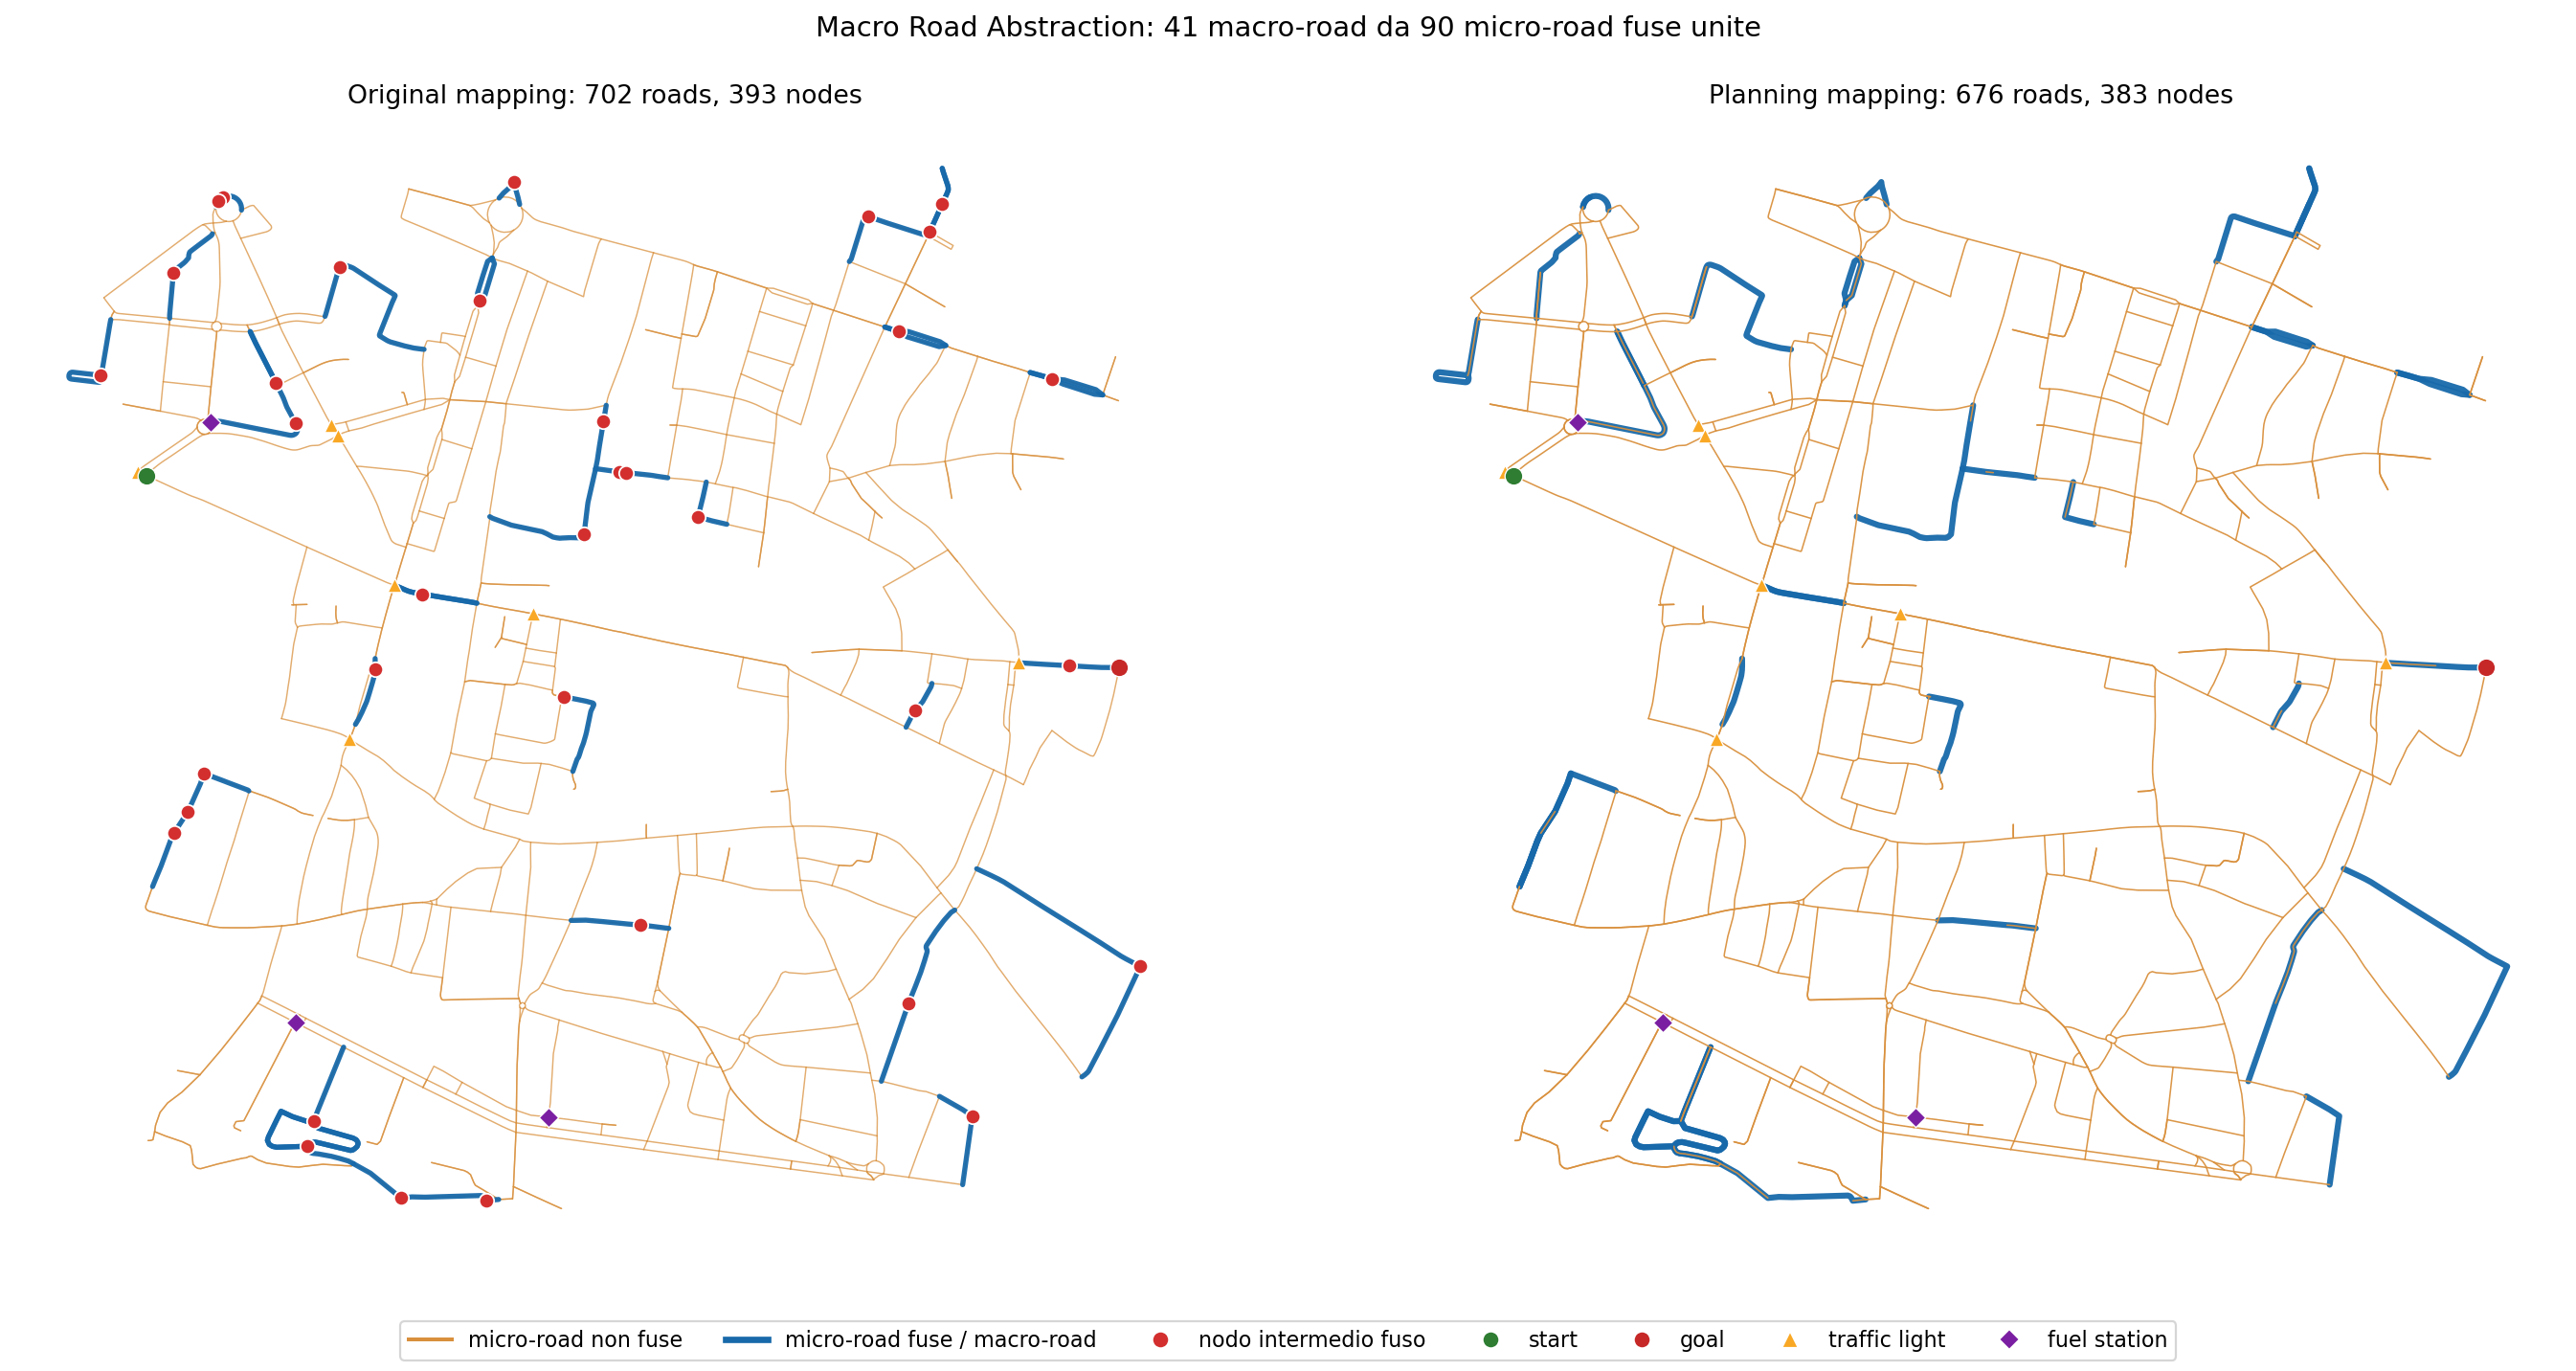
\includegraphics[width=0.88\linewidth]{macro_roads_comparison.png}
  \caption{Macro-road abstraction in the verified Bologna 500-node case. The
  planning representation changes from 702 roads and 393 nodes to 676 roads
  and 383 nodes; 90 micro-roads are grouped into 41 macro-roads. The modest
  reduction reflects the need to preserve many real decision points.}
  \label{fig:macro}
\end{figure}

\subsection{Controller-side scalability branch}
The second branch preserves the canonical
\texttt{process + node\_based + parameterized} model. Scalability is obtained
outside a single planner call: Python generates smaller problems, invokes
ENHSP repeatedly, executes a node-consistent prefix, updates global state, and
concatenates the partial plans. The two branches are complementary rather than
stacked: compiled traversal simplifies the model given to the planner, whereas
the controller retains the expressive process model and reduces the horizon of
each call.

\begin{figure}[H]
\centering
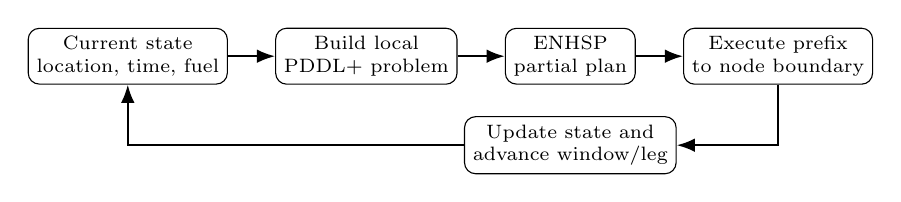
\begin{tikzpicture}[
  node distance=4mm and 6mm,
  box/.style={draw,rounded corners,align=center,minimum height=6mm,inner sep=3pt,font=\scriptsize},
  arr/.style={-Latex,thick}
]
\node[box] (state) {Current state\\location, time, fuel};
\node[box,right=of state] (problem) {Build local\\PDDL+ problem};
\node[box,right=of problem] (plan) {ENHSP\\partial plan};
\node[box,right=of plan] (prefix) {Execute prefix\\to node boundary};
\node[box,below=of plan] (update) {Update state and\\advance window/leg};
\draw[arr] (state) -- (problem);
\draw[arr] (problem) -- (plan);
\draw[arr] (plan) -- (prefix);
\draw[arr] (prefix.south) |- (update.east);
\draw[arr] (update.west) -| (state.south);
\end{tikzpicture}
\caption{Controller-side plan--execute-prefix--update loop.}
\label{fig:controller-loop}
\end{figure}

The \textbf{congestion controller} divides time into windows. For each window it
computes one static congestion snapshot, generates a process-model problem from
the current location to the unchanged final goal, and executes the last
completed traversal that fits the window. A node-boundary rule prevents the
next problem from inventing a location while the vehicle is still on a road.
Across iterations the congestion profile is dynamic, although each individual
PDDL problem is static.

The \textbf{fuel controller} decomposes the route by reachability. If the final
goal is reachable with current fuel, it remains the planning target; otherwise
the controller selects a reachable fuel station according to its station
policy, solves that leg, updates fuel, and continues until the final goal is
reached. Fuel and congestion replanning are currently mutually exclusive.

\section{Route-Unaware LLM Event Injection}
The LLM is not used as the route planner. Classical planners are more reliable
for feasibility once a formal problem is available, whereas standalone LLMs
remain inconsistent on long-horizon planning tasks \cite{liu2023,valmeekam2023}.
Routly uses the LLM as a constrained generator of \emph{exogenous events}.
First, ENHSP produces a baseline plan
\[
  P_0=\operatorname{Plan}(G,s,g).
\]
The LLM then receives valid road identifiers, the incident nodes of each road,
$s$ and $g$, and optional geometric information, but it does not receive
$P_0$. It returns structured closures or slowdowns. A closure changes
\texttt{road-open}; a slowdown changes the congestion factor used to compute
travel duration. After schema and topology validation, the modified graph
$G_E$ is planned again from the same initial state:
\[
  P_1=\operatorname{Plan}(G_E,s,g).
\]
This is a counterfactual second planning run, not online replanning from a
vehicle position reached during $P_0$.

Two candidate-selection modes are implemented. With
\texttt{strategic\_injection=false}, the LLM receives a reproducible random
subset of at most 120 roads. With it enabled, Python extracts a corridor around
the straight start-goal axis and supplies each candidate road's distance from
that axis, encouraging disruptions on plausible corridors without revealing
the baseline plan. Consequently, route-hit performance measures the combined
geometric filter and LLM choice, not the LLM alone. A solvability guard can
convert path-breaking closures into slowdowns (or skip them); raw event quality
and post-guard planning success must therefore be reported separately.

\begin{figure}[H]
\centering
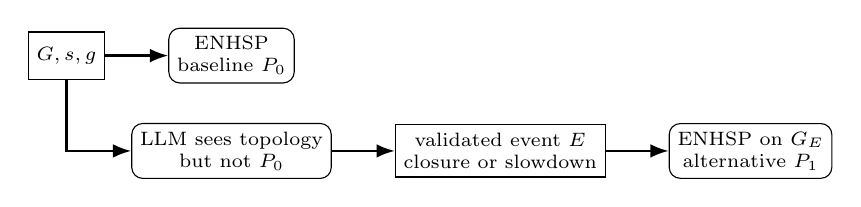
\begin{tikzpicture}[
  node distance=5mm and 8mm,
  box/.style={draw,rounded corners,align=center,minimum height=6mm,inner sep=3pt,font=\scriptsize},
  data/.style={draw,align=center,minimum height=6mm,inner sep=3pt,font=\scriptsize},
  arr/.style={-Latex,thick}
]
\node[data] (g) {$G,s,g$};
\node[box,right=of g] (p0) {ENHSP\\baseline $P_0$};
\node[box,below=of p0] (llm) {LLM sees topology\\but not $P_0$};
\node[data,right=of llm] (event) {validated event $E$\\closure or slowdown};
\node[box,right=of event] (p1) {ENHSP on $G_E$\\alternative $P_1$};
\draw[arr] (g) -- (p0);
\draw[arr] (g.south) |- (llm.west);
\draw[arr] (llm) -- (event);
\draw[arr] (event) -- (p1);
\end{tikzpicture}
\caption{Plan-hidden event generation and second planning run.}
\label{fig:llm-protocol}
\end{figure}

\section{Results and Experimental Protocol}
All comparisons must fix the map seed, graph crop, start/goal pair, background
traffic, Java heap, ENHSP version, and feature configuration. Each run archives
the resolved YAML, domain, problem, solver log, plan, macro expansion when
applicable, event JSON, and SUMO output. The full campaign spans the five
planner formulations over increasing graph sizes, macro-road on/off,
static/dynamic/hybrid congestion, the two controllers, and fuel modes. This
draft reports only measurements already verified in the supplied logs; missing
aggregate results are explicitly marked rather than inferred.

\subsection{RQ1: verified model-side evidence}
Table~\ref{tab:verified} isolates the grounding intervention on one Bologna
case with 677 planning roads, 384 locations, 14 global windows, and 8~GB Java
heap. The generic encoding has a compact domain, but its type-compatible upper
bound is about $1.50\times10^9$ assignments. The hard-coded road-specific
attempt demonstrates that syntactically valid PDDL is not sufficient for a
particular grounder. Singleton types retain standard PDDL parameters while
restricting each to one legal object, converting an out-of-memory failure into
a solved instance.

\begin{table}[H]
\centering
\caption{Verified grounding reformulation result on the same 500-node case.}
\label{tab:verified}
\scriptsize
\begin{tabularx}{\linewidth}{@{}p{2.35cm}Y p{1.75cm}p{3.15cm}@{}}
\toprule
Encoding & Symbolic exposure & ENHSP outcome & Measured evidence \\
\midrule
Generic parameterized & Two schemas; upper bound $677\cdot384^2\cdot(1+14)\approx1.50\times10^9$ & Grounding failed & Java OOM after about 45.1~s; no plan. \\
Road-specific hard-coded & 3927 schemas, only vehicle parameter & Grounding unreliable & $|A|=0$ in minimal tests; large case declared unsolvable. \\
Road-specific singleton & 427 static + 3500 dynamic schemas & Solved & Grounding 4.117~s; $|A|=3858$; $|E|=13$; search 12.039~s; plan length 14. \\
\bottomrule
\end{tabularx}
\end{table}

A later hybrid calibration used 676 macro roads, 14 windows, and selected 69
dynamic roads at $\theta=0.10$. It generated 607 static plus 966 dynamic action
schemas, grounded in 1.609~s, and completed search in 6.539~s with a 15-step
plan. Thresholds above the observed temporal range collapsed hybrid to a static
case, whereas $\theta=0.05$ selected 341 roads and increased runtime to about
20.7~s. The selected threshold is therefore an empirical trade-off, not a
universal constant. Macro-road abstraction itself reduced topology only from
702/393 roads/nodes to 676/383; its value is correctness-preserving reduction,
not a claim of dramatic compression on every urban graph.

\subsection{RQ2: controller evaluation to consolidate}
The controller comparison must be performed within the process formulation:
process without controller versus process with congestion snapshots, and
process with direct fuel versus the fuel controller. Required metrics are the
number of planner calls, total grounding/search time, maximum per-call memory,
number of partial plans, final plan metric, and SUMO-valid route completion.
The final table should report the same graph sizes used for RQ1 and must not
compare a controller's sum of local calls directly with compiled duration
without explaining their different semantics.

\begin{table}[H]
\centering
\caption{Controller results to populate from the consolidated experiment archive.}
\label{tab:controller-results}
\scriptsize
\begin{tabularx}{\linewidth}{@{}p{3.0cm}c c Y@{}}
\toprule
Configuration & Calls & Total planner time & Evidence to report \\
\midrule
Process baseline & \textit{[fill]} & \textit{[fill]} & Single monolithic plan, peak memory, final metric, SUMO validity. \\
Congestion controller & \textit{[fill]} & \textit{[fill]} & Number of windows, node-boundary prefixes, final metric, SUMO validity. \\
Fuel controller & \textit{[fill]} & \textit{[fill]} & Number of station legs, refuels, final metric, SUMO validity. \\
\bottomrule
\end{tabularx}
\end{table}

\subsection{RQ3: LLM disruption quality}
The LLM study should use a fixed set of graph instances and repeated seeds for
both random and strategic candidate selection. The core measures are: (i)
valid-event rate, (ii) baseline-route hit rate although $P_0$ is hidden, (iii)
planning success after the raw event and after the solvability guard, (iv) road
or distance overlap between $P_0$ and $P_1$, and (v) added travel cost. This
turns the vague question of whether the LLM is ``intelligent'' into a
measurable study of valid, route-relevant perturbation.

\figureplaceholder{0.105\textheight}{Replace this box with one representative
Bologna experiment showing the baseline route, the event roads/intersections,
and the post-event route. Use a no-fuel run so route changes are attributable
to the LLM event rather than refuelling.}{Representative pre/post route under a
route-unaware LLM disruption.}

\section{Conclusions and Future Work}
Routly frames urban routing as a declarative planning problem whose realism and
scalability are in direct tension. Congestion, signal timing, fuel, and road
availability can be described in PDDL/PDDL+, but a generic road-location-window
encoding can overwhelm grounding before search begins. The main contribution
is therefore not a new universal shortest-path algorithm; it is a reproducible
study of how domain-specific reformulation changes the tractability of
expressive urban planning. Model-side compilation removes unnecessary mid-road
state, road- or transition-specific singleton types prevent unrelated objects
from forming a Cartesian product, hybrid windows retain temporal variation
selectively, and macro roads reduce topology without losing the mapping to
SUMO. Controller-side planning provides a complementary path: it preserves the
process model while distributing a global route across smaller, state-linked
planner calls. The LLM layer remains outside the correctness-critical search
and instead generates validated, plan-hidden disruptions that test route
adaptation.

The strongest verified result is the transition from an out-of-memory generic
encoding to a complete singleton-typed plan on the same 500-node case. The
principal limitation of this draft is that the full multi-size controller and
LLM experiment matrices still need to be consolidated into the final tables.
Further work should combine the currently exclusive controllers in one
hierarchy: fuel selects the temporary target, congestion determines the
window-specific road costs, ENHSP selects the route, and Python updates
location, time, fuel, and refuelling before the next call. Additional work
includes mid-road controller state restoration, evaluation on cities with
contrasting topology, and online injection of events after a prefix of the
baseline route has actually been executed.

\vspace{-0.35em}
\begin{multicols}{2}
\begin{thebibliography}{99}\scriptsize

\bibitem{foxlong2006}
M. Fox and D. Long, ``Modelling Mixed Discrete-Continuous Domains for
Planning,'' \emph{Journal of Artificial Intelligence Research}, vol. 27,
pp. 235--297, 2006. \url{https://doi.org/10.1613/jair.2044}

\bibitem{scala2016}
E. Scala, P. Haslum, S. Thi\'ebaux, and M. Ram\'irez, ``Interval-Based
Relaxation for General Numeric Planning,'' in \emph{Proc. ECAI}, pp. 655--663,
2016. \url{https://users.cecs.anu.edu.au/~thiebaux/papers/ecai16.pdf}

\bibitem{vallati2016}
M. Vallati, D. Magazzeni, B. De Schutter, L. Chrpa, and T. L. McCluskey,
``Efficient Macroscopic Urban Traffic Models for Reducing Congestion: A PDDL+
Planning Approach,'' in \emph{Proc. AAAI}, pp. 3188--3194, 2016.
\url{https://ojs.aaai.org/index.php/AAAI/article/view/10399}

\bibitem{franco2019}
S. Franco, M. Vallati, A. Lindsay, and T. L. McCluskey, ``Improving Planning
Performance in PDDL+ Domains via Automated Predicate Reformulation,'' in
\emph{Computational Science -- ICCS 2019}, pp. 491--498, 2019.
\url{https://doi.org/10.1007/978-3-030-22750-0_42}

\bibitem{piotrowski2024}
W. Piotrowski and A. Perez, ``Real-World Planning with PDDL+ and Beyond,''
\emph{arXiv:2402.11901}, 2024.
\url{https://arxiv.org/abs/2402.11901}

\bibitem{micheli2026}
A. Micheli, E. Scala, and A. Valentini, ``Compiling Temporal Numeric Planning
into Discrete PDDL+: Extended Version,'' \emph{arXiv:2603.12188}, 2026.
\url{https://arxiv.org/abs/2603.12188}

\bibitem{baum2015}
M. Baum, J. Dibbelt, T. Pajor, and D. Wagner, ``Dynamic Time-Dependent Route
Planning in Road Networks with User Preferences,'' \emph{arXiv:1512.09132},
2015. \url{https://arxiv.org/abs/1512.09132}

\bibitem{liu2023}
B. Liu, Y. Jiang, X. Zhang, Q. Liu, S. Zhang, J. Biswas, and P. Stone,
``LLM+P: Empowering Large Language Models with Optimal Planning Proficiency,''
\emph{arXiv:2304.11477}, 2023.
\url{https://arxiv.org/abs/2304.11477}

\bibitem{valmeekam2023}
K. Valmeekam, M. Marquez, S. Sreedharan, and S. Kambhampati, ``On the
Planning Abilities of Large Language Models: A Critical Investigation,''
\emph{arXiv:2305.15771}, 2023.
\url{https://arxiv.org/abs/2305.15771}

\bibitem{boeing2017}
G. Boeing, ``OSMnx: New Methods for Acquiring, Constructing, Analyzing, and
Visualizing Complex Street Networks,'' \emph{Computers, Environment and Urban
Systems}, vol. 65, pp. 126--139, 2017.
\url{https://doi.org/10.1016/j.compenvurbsys.2017.05.004}

\bibitem{boeing2025}
G. Boeing, ``Modeling and Analyzing Urban Networks and Amenities with OSMnx,''
\emph{Geographical Analysis}, vol. 57, no. 4, pp. 567--577, 2025.
\url{https://doi.org/10.1111/gean.70009}

\bibitem{lopez2018}
P. Alvarez Lopez et al., ``Microscopic Traffic Simulation using SUMO,'' in
\emph{2018 21st International Conference on Intelligent Transportation
Systems}, pp. 2575--2582, 2018. \url{https://elib.dlr.de/127994/}

\bibitem{nardino2021}
M. Nardino, L. Cremonini, T. Georgiadis, E. Mandanici, and G. Bitelli,
``Microclimate Classification of Bologna (Italy) as a Support Tool for Urban
Services and Regeneration,'' \emph{International Journal of Environmental
Research and Public Health}, vol. 18, no. 9, art. 4898, 2021.
\url{https://doi.org/10.3390/ijerph18094898}

\bibitem{routlycode}
G. Rudi et al., ``Routly Planner source code and reproducible experiment
artefacts,'' 2026. \url{https://github.com/GiuseppeRudi/routly-planner}

\end{thebibliography}
\end{multicols}

\end{document}
